%4
\section{Konkrete Architektur}

Abbildung \ref{KomponentendiagrammKonkret} zeigt die Komponenten \emph{ServerSoftware} und \emph{RobotSoftware} in einem Komponentendiagramm.

\begin{figure}[H]
\centering
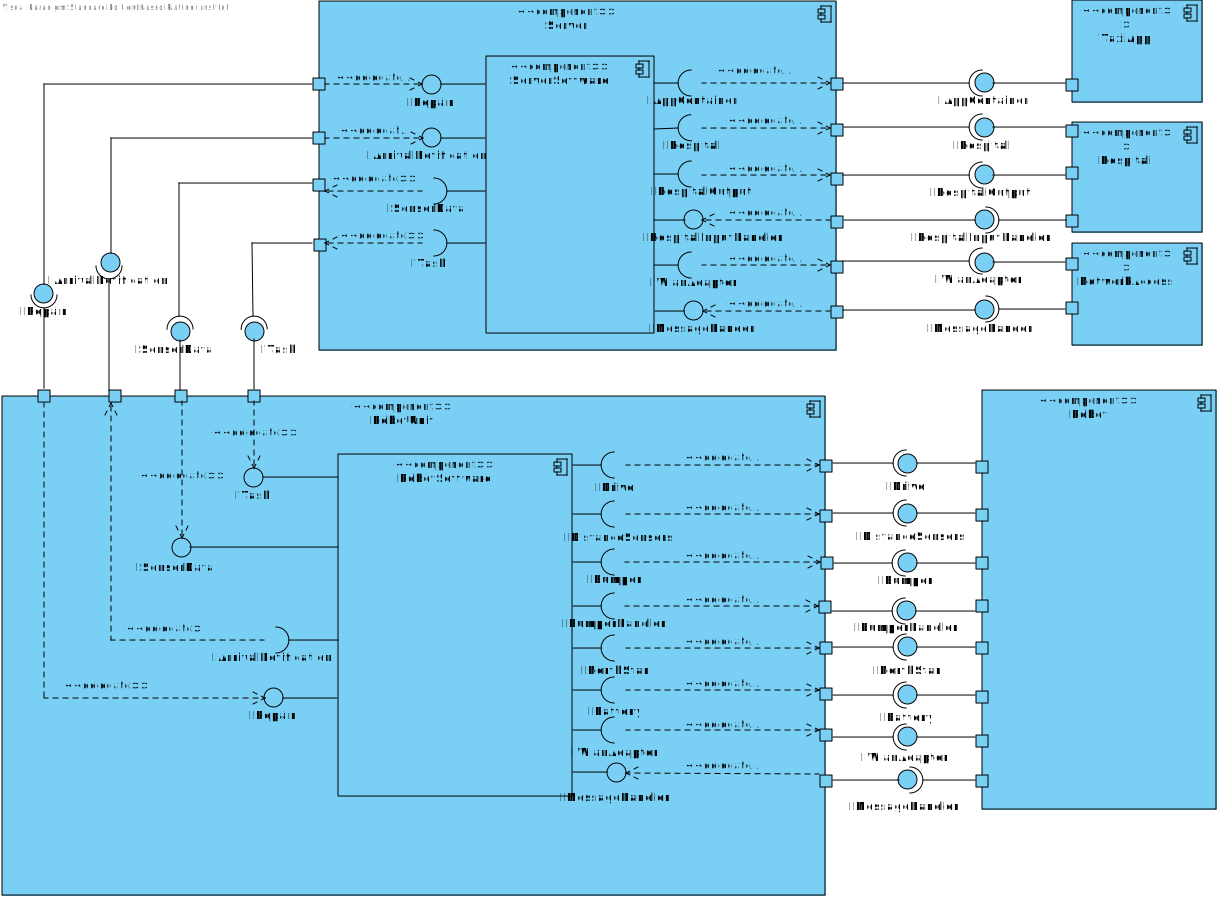
\includegraphics[width=1\textwidth]{img/2-Entwurf-4-KonkreteArchitektur}
\caption{Komponentendiagramm mit den Komponenteninterfaces}
\label{KomponentendiagrammKonkret}
\end{figure}

%4.1 Server Software
\subsection{\textit{ServerSoftware}}

Die \emph{ServerSoftware} spricht den \textit{Robot} über dessen \textit{IWlanAdapter} an,
um den besten \textit{Robot} für eine \textit{Destination} zu ermitteln und einem \textit{Robot} eine \textit{Destination} zuzuweisen.

%4.2 Robot Software
\subsection{\textit{RobotSoftware}}

\emph{RobotSoftware} ist für die Steuerung der \textit{RobotUnit} zuständig. 
Die von der abstrakten Hardware
des \textit{Robot} angebotenen, vorgegebenen Interfaces \textit{INorthStar, IBattery, IDrive, IDistanceSensors, IBumper} sowie
\textit{IBumperHandler} werden dabei von der \textit{Robot}-Komponente für die konkrete Steuerung der \textit{RobotUnit} genutzt.
